\documentclass{article}
\usepackage{../almeida}

\begin{document}
Name:\ \makebox[4in]{\hrulefill} \hspace{1in} Date:\ \makebox[1in]{\hrulefill}
\begin{center}
    \textbf{PS-01: $\epsilon-\delta$ Proofs, Part I}
\end{center}

% A customized box with a title and colors
\begin{center}
\begin{tcolorbox}[colback=white, colframe=black, colbacktitle=white, coltitle=black, title=\textbf{Topics},boxrule=1pt,width=12cm]
    \begin{itemize}
      \item Introduction to $\epsilon-\delta$ definition of a limit
      \item $\epsilon-\delta$ limits of linear function
    \end{itemize}
\end{tcolorbox}
\end{center}

\begin{enumerate}
\item In the following exercises, use the graphs to find a $\delta > 0$ such that for all $x$,
\begin{equation*}
0 < \left|x-c\right| < \delta \implies \left| f(x) - L \right| < \epsilon
\end{equation*}
\begin{tabular}{p{8cm} p{8cm}}
  (a) & (b) \\
  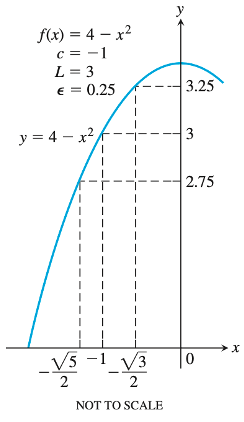
\includegraphics{1a.png} & 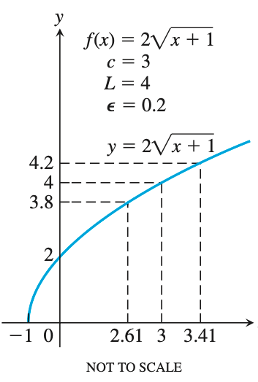
\includegraphics{1b.png} \\
\end{tabular}
% Source: Thomas' Calculus, 13th Edition, Problems 2.3.10 and 2.3.12

\item Each of the following exercises gives a function $f(x)$ and numbers $L$, $c$, and $\epsilon>0$. In each case, find an open interval about $c$ on which the inequality $\left| f(x) - L\right| < \epsilon$ holds. Then, give a value for $\delta > 0$ such that for all $x$ satisfying $0 < \left|x-c\right| < \delta$, the inequality $\left| f(x) - L\right| < \epsilon$ holds. \newline

{\centering
\renewcommand{\arraystretch}{1.5}
\begin{tabular}{|c|l|l|l|l|}
  \hline
  (a) & $f(x)=2x-2$ & $L=-6$ & $c=-2$ & $\epsilon=0.02$ \\
  \hline
  (b) & $f(x)=\sqrt{x+1}$ & $L=1$ & $c=0$ & $\epsilon=0.1$ \\
  \hline
\end{tabular}
\vspace{0.5cm} \par
}
\item Give an $\epsilon-\delta$ prove of each stated fact
      \begin{tasks}
        \task $\lim_{x \to 0} \left(2x-1\right)=-1$
        \task $\lim_{x \to 0} \left(3x-3\right) = -64$
        \task $\lim_{x \to c} \left(mx+b\right) = mc+b$
      \end{tasks}
\end{enumerate}

\pagebreak
\subsection{Solutions}
\begin{enumerate}
\item This is is from Thomas 2.3.16
\end{enumerate}

\begin{align*}
	\left| (2x-2) - (-6) \right| &< 0.02 \\
	 \left| 2x +4 \right| 	 &< 0.02 \\
	-0.02 < 2x+4 &< 0.02 \\
	-4.02 < 2x &< 3.98 \\
	-2.01 < x &< 1.99
\end{align*}

\textbf{3c}
\begin{proof}
  Let $\epsilon > 0$ be given. We need to find a $\delta > 0$ such that for all $x$,
  \begin{equation*}
    0 < |x - c| < \delta \implies |f(x) - L| < \epsilon
  \end{equation*}
  Let $\varepsilon>0$ and choose $\delta = \frac{\varepsilon}{\left|m\right|}$. Then,
  
  \begin{align*}
    |f(x) - L| &= |(mx + b) - (mc + b)| \\
                 &= |mx - mc| \\
                 &= |m|\cdot\underbrace{|x-c|}_{< \delta}
  \end{align*}
  
  To ensure that $|f(x) - L| < \epsilon$, we need:
  \begin{equation*}
    |m||x - c| < \epsilon
  \end{equation*}
  
  If $m \neq 0$, we can choose $\delta = \frac{\epsilon}{|m|}$. Then, for all $x$ satisfying $0 < |x - c| < \delta$, we have:
  \begin{equation*}
    |f(x) - L| = |m||x - c| < |m| \cdot \frac{\epsilon}{|m|} = \epsilon
  \end{equation*}
  
  Therefore, $\lim_{x \to c} (mx + b) = mc + b$.
\end{proof}

% Figure for the graph of f(x) = 4 - x^2 ======================== 
\begin{tikzpicture}[scale=1.5]
    % Colors
    \definecolor{curveblue}{RGB}{0, 150, 215}

    % Axes
    \draw[->, thick] (-3.5, 0) -- (1, 0) node[right] {$x$};
    \draw[->, thick] (0, -0.4) -- (0, 4.8) node[above] {$y$};
    \node[below right] at (0, 0) {$0$};

    % Function definition parameters
    % f(x) = 4 - x^2
    % Points:
    % x = -sqrt(5)/2 approx -1.118 -> y = 2.75
    % x = -1                       -> y = 3.00
    % x = -sqrt(3)/2 approx -0.866 -> y = 3.25

    % Labels top left
    % \node[anchor=west] at (-3.2, 4.4) {$f(x)=4-x^2$};
    % \node[anchor=west] at (-2.8, 4.0) {$c = -1$};
    % \node[anchor=west] at (-2.8, 3.6) {$L = 3$};
    % \node[anchor=west] at (-2.8, 3.2) {$\epsilon = 0.25$};
    \node[anchor=west] at (-2.5, 3.8) {
      $\begin{aligned}
        f(x) &= 4 - x^2 \\
        c &= -1 \\
        L &= 3 \\
        \epsilon &= 0.25 \\
      \end{aligned}$};

    % Label for curve
    \node[left] at (-1.75, 1.0) {$y = 4 - x^2$};

    % Dashed lines and ticks
    % x = -sqrt(5)/2 , y = 2.75
    \draw[dashed, thick, gray!80!black] ({-sqrt(5)/2}, 0) -- ({-sqrt(5)/2}, 2.75) -- (0, 2.75);
    % x = -1 , y = 3
    \draw[dashed, thick, gray!80!black] (-1, 0) -- (-1, 3) -- (0, 3);
    % x = -sqrt(3)/2 , y = 3.25
    \draw[dashed, thick, gray!80!black] ({-sqrt(3)/2}, 0) -- ({-sqrt(3)/2}, 3.25) -- (0, 3.25);
    \draw[solid, thin, gray!80!black] ({-sqrt(3)/2},0) -- ({-sqrt(3)/2+0.35},-0.15);
    \draw[solid, thin, gray!80!black] ({-sqrt(5)/2},0) -- ({-sqrt(5)/2-0.35},-0.15);

    % Axis Labels
    % Y-axis labels
    \node[right] at (0, 3.25) {$3.25$};
    \node[right] at (0, 3.0) {$3$};
    \node[right] at (0, 2.75) {$2.75$};

    % X-axis labels
    \node[below, thick, font=\small, anchor=north] at ({-sqrt(5)/2-0.5}, -0.1) {$-\frac{\sqrt{5}}{2}$};
    \node[below, font=\small] at (-1, -0.05) {$-1$};
    \node[below, thick, font=\small,anchor=north] at ({-sqrt(5)/2+0.5}, -0.1) {$-\frac{\sqrt{3}}{2}$};

    % Not to scale caption
    \node at (-1.2, -1.0) {\small \textbf{NOT TO SCALE}};

    % Plot parabola
    \draw[cyan!80!blue, ultra thick, domain=-2:0.5, samples=100] plot (\x, {4 - (\x)^2});

\end{tikzpicture}

% Figure for the graph of f(x) = 2*sqrt(x+1) ========================
\begin{tikzpicture}[scale=1.5]
    % Colors
    \definecolor{curveblue}{RGB}{0, 150, 215}

    % Axes
    \draw[->, thick] (0, -0.4) -- (0, 4.8) node[above] {$y$};
    \draw[->, thick] (-2.0, 0) -- (4, 0) node[right] {$x$};
    \node[below right] at (0, 0) {$0$};

    % Function definition parameters
    % f(x) = 4 - x^2
    % Points:
    % x = -sqrt(5)/2 approx -1.118 -> y = 2.75
    % x = -1                       -> y = 3.00
    % x = -sqrt(3)/2 approx -0.866 -> y = 3.25

    % Labels top left
    % \node[anchor=west] at (-3.2, 4.4) {$f(x)=4-x^2$};
    % \node[anchor=west] at (-2.8, 4.0) {$c = -1$};
    % \node[anchor=west] at (-2.8, 3.6) {$L = 3$};
    % \node[anchor=west] at (-2.8, 3.2) {$\epsilon = 0.25$};
    \node[anchor=west] at (-2, 1.75) {
      $\begin{aligned}
        f(x) &= 2\sqrt{x+1} \\
        c &= 3 \\
        L &= 4 \\
        \epsilon &= 0.2 \\
      \end{aligned}$};

    % Label for curve
    \node[left] at (2.2, 2.5) {$y = 2\sqrt{x+1}$};

    % Dashed lines and ticks
    \draw[dashed, thick, gray!80!black] (2.61, 0) -- (2.61,3.8) -- (0, 3.8);
    \draw[dashed, thick, gray!80!black] (3, 0) -- (3, 4) -- (0, 4);
    \draw[dashed, thick, gray!80!black] (3.41, 0) -- (3.41, 4.2) -- (0, 4.2);
    % \draw[solid, thin, gray!80!black] ({-sqrt(3)/2},0) -- ({-sqrt(3)/2+0.35},-0.15);
    % \draw[solid, thin, gray!80!black] ({-sqrt(5)/2},0) -- ({-sqrt(5)/2-0.35},-0.15);

    % Axis Labels
    % Y-axis labels
    \node[right] at (-0.45, 4.2) {$4.2$};
    \node[right] at (-0.45, 4) {$4$};
    \node[right] at (-0.45, 3.8) {$3.8$};

    % X-axis labels
    \node[below, thick] at (2.5, -0.05) {2.61};
    \node[below, thick] at (3, -0.05) {$3$};
    \node[below, thick] at (3.50, -0.05) {3.41};
    % \node[below, thick, font=\small, anchor=north] at ({-sqrt(5)/2-0.5}, -0.1) {$-\frac{\sqrt{5}}{2}$};
    % \node[below, font=\small] at (-1, -0.05) {$-1$};
    % \node[below, thick, font=\small,anchor=north] at ({-sqrt(5)/2+0.5}, -0.1) {$-\frac{\sqrt{3}}{2}$};

    % Not to scale caption
    \node at (1.3, -0.7) {\small \textbf{NOT TO SCALE}};

    % Plot parabola
    \draw[cyan!80!blue, ultra thick, domain=-1:4, samples=1000] plot (\x, {2*sqrt(\x+1)});

\end{tikzpicture}

\begin{figure}[H]
\centering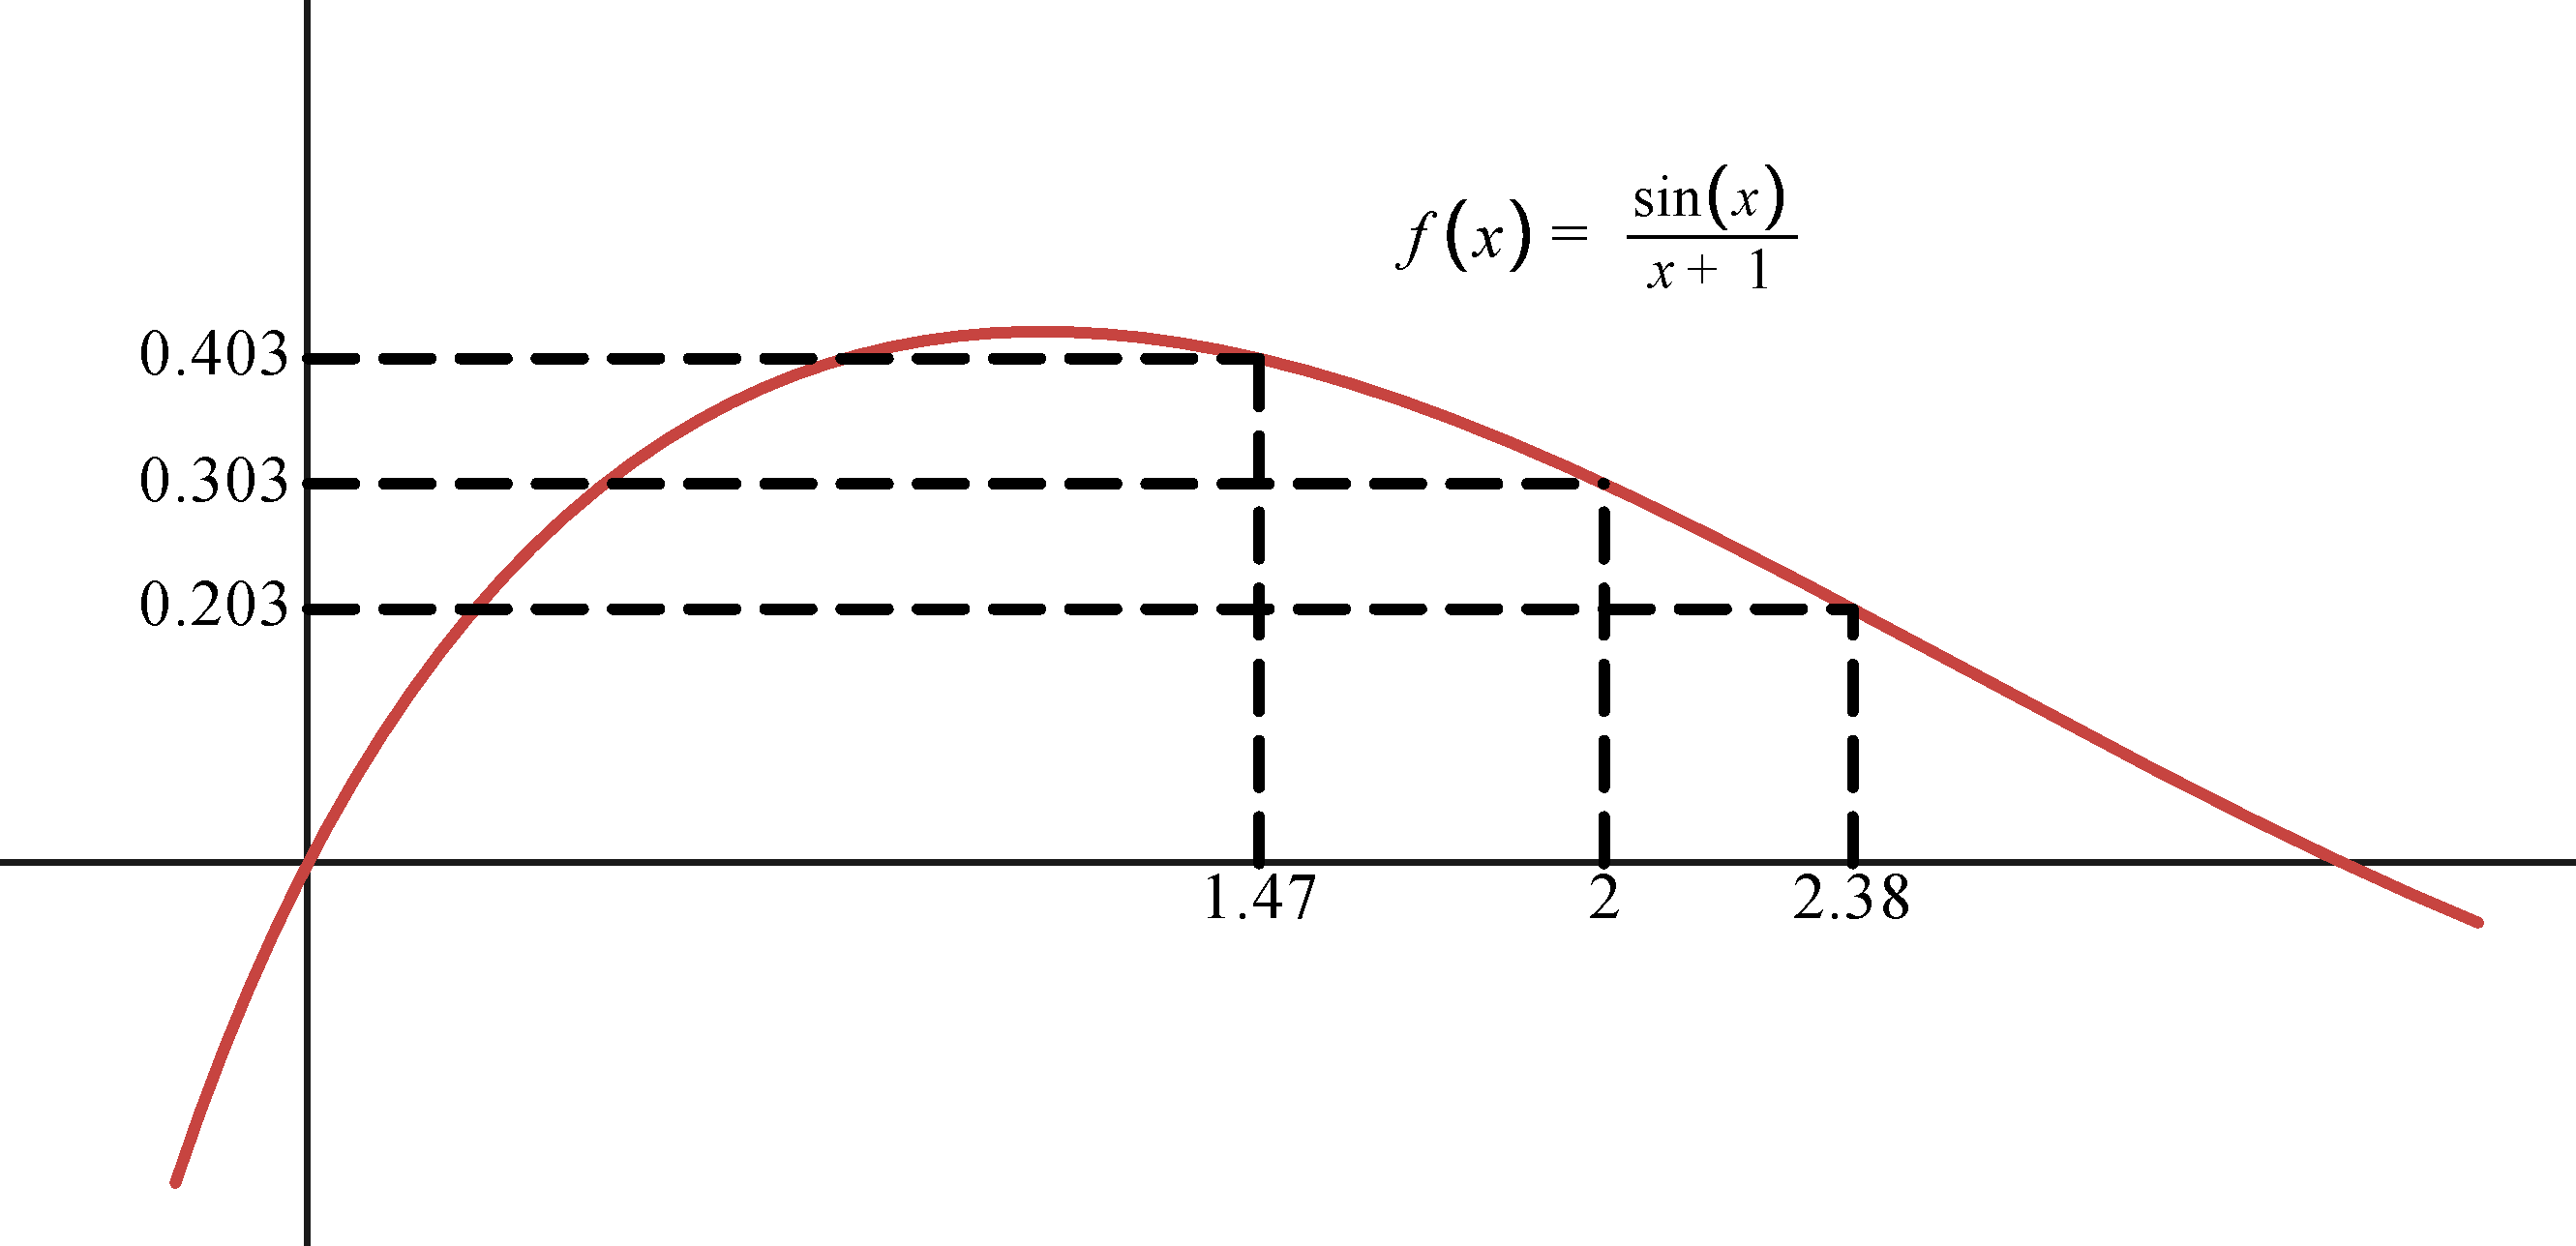
\includegraphics[width=8cm]{desmos-13.pdf}
\caption{\url{https://www.desmos.com/calculator/vpiohuxekz}}
\end{figure}
\end{document}